\documentclass[lettersize,journal]{IEEEtran}
\IEEEoverridecommandlockouts

% Packages (follow IEEE official template)
\usepackage[T1]{fontenc}
\usepackage[noadjust]{cite}
\usepackage{amsmath,amssymb,amsfonts}
\usepackage{amsthm}
\renewcommand{\qedsymbol}{$\blacksquare$}
\renewcommand{\proofname}{\bfseries Proof}
\makeatletter
\renewenvironment{proof}[1][\proofname]{\par
  \pushQED{\qed}%
  \normalfont \topsep6\p@\@plus6\p@\relax
  \trivlist
  \item[\hskip\labelsep
        \itshape
  #1\@addpunct{:}]\ignorespaces
}{%
  \popQED\endtrivlist\@endpefalse
}
\makeatother
\usepackage{algorithmic}
\usepackage{algorithm}
\usepackage{array}
\usepackage{textcomp}
\usepackage{stfloats}
\usepackage{placeins}
\usepackage{dblfloatfix}
\usepackage{balance}
\usepackage{float}
\raggedbottom
\hfuzz=5pt
\tolerance=10000
\emergencystretch=3em
\usepackage{url}
\usepackage{graphicx}
\usepackage{booktabs}
\usepackage{multirow}
\usepackage{hyperref}

\hyphenation{op-tical net-works semi-conduc-tor IEEE-Xplore}

% Theorem environments (numbered within sections)
\newtheorem{theorem}{Theorem}
\newtheorem{lemma}[theorem]{Lemma}
\newtheorem{definition}[theorem]{Definition}

% Custom commands
\newcommand{\ie}{\textit{i.e.,}}
\newcommand{\eg}{\textit{e.g.,}}
\newcommand{\etal}{\textit{et al.}}
\newcommand{\etc}{\textit{etc.}}
\newcommand{\cf}{\textit{cf.}}
\newcommand{\vs}{\textit{vs.}}
\newcommand{\wrt}{\textit{w.r.t.}}

\title{Time-Aware CP-ABE with Threshold Policies for Digital Twin Security in Industrial IoT}

\author{
\IEEEauthorblockN{Xinkai Yang$^{1}$ and He Xiao$^{1}$}
\IEEEauthorblockA{
$^{1}$School of Industrial Software,\\
Jiangxi University of Science and Technology,\\
Nanchang, China\\
Email: y13517096949@qq.com}
}

\begin{document}

\markboth{IEEE Internet of Things Journal}%
{Yang \MakeLowercase{\textit{et al.}}: Time-Aware CP-ABE with Threshold Policies for Digital Twin Security}

\maketitle

\begin{abstract}
Existing ciphertext-policy attribute-based encryption schemes for industrial
IoT digital twins lack native temporal access control, flexible threshold
policies, and efficient attribute revocation in a unified framework, leaving
systems vulnerable to time-based and privilege-escalation attacks.
We propose T-CP-ABE, a time-aware CP-ABE framework that natively integrates
$k$-of-$n$ THRESHOLD gates and version-based attribute revocation with
forward security: temporal access control is enforced through LSSS policy
attributes with hash-chain forward security, while BLS signatures and a
conditional diffusion model provide complementary authentication and
anomaly detection layers.
We formalize the IND-sCPA-T security model---a security proof that
incorporates both temporal token queries and
attribute-version revocation queries within a unified adversary
model---and prove security under the DBDH assumption.
Implemented in Charm-Crypto, the framework achieves sub-300\,ms decryption
for typical IoT policies ($\leq$10 attributes) with key-generation
performance stable across 10--10,000 user attributes, and linear policy
scaling (23.6\,s at 1000 policy attributes) acceptable for offline batch
audit. Validation on UNSW-NB15 and four real-world
scenarios confirms practical applicability for industrial digital twin
deployments.
\end{abstract}

\begin{IEEEkeywords}
Attribute-based encryption, time-aware access control, digital twin, industrial IoT, threshold policy
\end{IEEEkeywords}

\section{Introduction}
\label{sec:introduction}

\IEEEPARstart{R}{ecently}, the convergence of digital twin technology and the Industrial
Internet of Things (IIoT) has markedly transformed manufacturing, healthcare,
and smart city infrastructure through virtual replicas of physical assets that
enable real-time monitoring, predictive maintenance, and lifecycle
management~\cite{Sharma2022, LiuM2021, Fuller2020_DT_Survey}. As these
deployments scale across thousands of heterogeneous devices and organizational
boundaries, securing access to twin data becomes critical---unauthorized
reading exposes industrial secrets, while unauthorized modification can
cascade into physical-world safety failures. Ciphertext-policy attribute-based
encryption (CP-ABE) embeds access policies
directly in ciphertexts and allows decryption only by users whose attributes
satisfy the policy, offering a natural fit for fine-grained access control in
such environments.

However, practical deployment of CP-ABE in IIoT digital twin scenarios is
hindered by the absence of three features that must operate in concert:
temporal access control, flexible threshold policies, and efficient attribute
revocation~\cite{Li2022_CPABE_Survey, Iqal2024,
Aouedi2025_IoTSurvey, Sharma2026_IoTSecurity}. Existing schemes
address these in isolation---Zhu et al.~\cite{Zhu2012} established temporal
access control via cryptographic integer comparisons, Liu et
al.~\cite{Liu2018_ACNS} combined time-based direct revocation with CP-ABE,
and Hur et al.~\cite{Hur2011} tackled attribute revocation---yet no
construction unifies all three. Combining these mechanisms introduces
interaction-induced attack vectors absent when each is analyzed in isolation:
a revoked-but-unexpired time token could forge a decryption path unless
version tags are checked alongside the hash chain; injecting time tokens as
additional Shamir shares would alter the polynomial degree and lower the
threshold, so time metadata must be bound orthogonally to the share structure;
an adversary holding $k{-}1$ shares, a valid time token, and a revoked key
could bypass version checks if the integration is not carefully designed.
These challenges demand a combined construction with a formal security model
capturing the joint behavior of all mechanisms.

To reconcile this tension, we propose T-CP-ABE, a time-aware CP-ABE framework
for digital twin security in IIoT. The contributions are as follows. We
present a construction that natively supports THRESHOLD$(k,n)$ gates and
version-based attribute revocation with forward security, where temporal
access control is enforced through time predicate rows in the LSSS matrix
with hash-chain-based forward security, and a publicly computable metadata
tag records the encryption period for auditability. We formalize the
IND-sCPA-T security model---a selective chosen-plaintext game extending
standard IND-sCPA with time token and revocation queries---and prove
security under the DBDH assumption with advantage bound $\text{Adv} \leq
2\,\text{Adv}^{\text{DBDH}} + (q_H + q_K + q_T)/p$. This security proof
incorporates both temporal token queries
and attribute-version revocation queries within a unified adversary
model, capturing interaction-induced attack vectors absent when each
mechanism is analyzed in isolation. We further integrate BLS
digital signatures~\cite{Burgos2024} for mutual authentication and
a conditional diffusion model~\cite{Tang2023, TabDDPM2023, Ho2020_DDPM} for
anomaly detection as complementary security layers. Evaluation
using Charm-Crypto demonstrates sub-300\,ms decryption for
typical IoT policies, stable performance scaling to 10,000 attributes, and
validation on the UNSW-NB15 dataset~\cite{Zoghi2024}
alongside four real-world deployment scenarios.

The remainder of this article is organized as follows. Section~\ref{sec:related}
reviews related work on CP-ABE, temporal access control, and digital twin
security. Section~\ref{sec:preliminaries} presents the mathematical
preliminaries. Section~\ref{sec:system} defines the system architecture,
threat model, and IND-sCPA-T security game.
Section~\ref{sec:construction} describes the T-CP-ABE construction and its
security proofs. Section~\ref{sec:performance} reports experimental results.
Section~\ref{sec:conclusion} concludes with limitations and future directions.

% ============================================================
\section{Related Work}
\label{sec:related}
% ============================================================

Sahai and Waters~\cite{Sahai2005} pioneered ABE by linking attributes to keys
and access structures to ciphertexts~\cite{Shruti2023}. Bethencourt et
al.~\cite{Bethencourt2007} realized the ciphertext-policy variant (CP-ABE),
and Waters~\cite{Waters2011} achieved full non-selective security via linear
secret sharing schemes. Subsequent work addressed decryption
outsourcing, multi-authority
constructions~\cite{DecentralisedMAABE2025, Zhang2026_MultiAuthority,
Penuelas2024_MultiAuthority, Datta2025_Decentralized}, attribute
revocation~\cite{Liu2023_Revocation, Ghopur2023}, pairing-free
constructions for resource-constrained IoT
devices~\cite{Guo2024, Zhang2024_TDSC}, and
lattice-based post-quantum
ABE~\cite{Gasparini2026_LatticeBenchmark, Li2022_CPABE_Survey}. However, these
schemes do not support temporal access control, and cloud-based offloading
remains impractical for the massive data volumes generated by IIoT devices.

Zhu et al.~\cite{Zhu2012} established temporal access control by combining
cryptographic integer comparisons with CP-ABE, enabling time-bound encryption
without a trusted clock. Liu et al.~\cite{Liu2018_ACNS} extended this with
time-based direct revocation, though without flexible threshold policies.
Hu \etal~\cite{Hu2024_TAAC} proposed a time-attribute-based access control
scheme for SDN-IoT environments. Cai \etal~\cite{Cai2023_TimeABE} and
Li \etal~\cite{Li2023_HierarchicalABE} further explored time-bound ABE with
outsourcing support. All treat time as an external constraint rather than an integral part of the
access structure, and neither provides forward security through hash chains.
Combining temporal predicates with revocation introduces interaction-induced
attack vectors---a revoked-but-unexpired token could forge a decryption path
unless version tags are checked alongside the hash chain---yet no existing
scheme addresses these interactions with a formal security model.

Digital twin security frameworks~\cite{Lu2020_DTSecurity,
Fuller2020_DT_Survey, Mun2025_DTSurvey, Alhamam2025_DTCyber} address encryption and integrity but lack
fine-grained, time-aware access control. Dai \etal~\cite{Dai2024_FGCS}
combined blockchain with CP-ABE for digital twin sharing without temporal
constraints or forward security. Hybrid AI-driven access control frameworks
have been proposed for IIoT environments~\cite{Shruti2023}, yet
runtime threat detection via machine
learning~\cite{Pang2021_AnomalySurvey} operates independently of cryptographic
enforcement, leaving a gap between detection and access
control~\cite{Iqal2024, Gharib2025_IoTPlatforms}. Recent AI-driven
security frameworks---Khan~et~al.~\cite{Khan2025_HybridABAC} proposed a
hybrid ABAC with ML-driven policy adjustment for IIoT, and
Rahman~et~al.~\cite{Rahman2025_TrustEdge} integrated ABAC with
federated learning for smart homes---but neither closes the loop from
anomaly detection to cryptographic policy adaptation. We also
acknowledge the limitations of our pairing-based construction:
pairing-free schemes~\cite{Chen2025_PairingFree} achieve lower
decryption cost but require trusted proxy assumptions incompatible with
our threat model; lattice-based post-quantum
ABE~\cite{Poomekum2025_Lattice, Bagchi2025_PostQuantum} remains
impractical for resource-constrained IIoT due to key and ciphertext
size overhead exceeding $10\times$; and multi-authority
extensions~\cite{YeLin2025_MultiAuthority, Datta2025_Decentralized,
Cini2025_LatticeMAABE} eliminate single-TA key escrow but introduce
coordination latency unsuitable for real-time twin synchronization.
These trade-offs define the applicability boundary of T-CP-ABE:
centralized IIoT deployments where temporal access control and threshold
policies are primary requirements. To address these gaps, we
propose T-CP-ABE, which unifies temporal predicates, THRESHOLD gates, and
version-based revocation in a single CP-ABE construction.

Compared with schemes addressing a subset of these requirements, T-CP-ABE
provides the following distinctions. W.r.t.\ ABE with
revocation~\cite{Liu2023_Revocation, Ghopur2023}, we additionally support
temporal predicates and THRESHOLD gates natively in the LSSS matrix.
W.r.t.\ time-bound ABE~\cite{Zhu2012, Liu2018_ACNS, Hu2024_TAAC}, we
integrate version-based attribute revocation with forward security.
W.r.t.\ multi-authority ABE~\cite{Datta2025_Decentralized,
Zhang2026_MultiAuthority, YeLin2025_MultiAuthority, Cini2025_LatticeMAABE},
our single-TA design trades decentralization
for simplicity, suitable for digital twin deployments with a centralized
trust anchor.
W.r.t.\ pairing-free ABE~\cite{Chen2025_PairingFree}, our pairing-based
construction targets IIoT devices with moderate computational capacity
where trusted proxy assumptions are unacceptable.
W.r.t.\ lattice-based post-quantum
ABE~\cite{Gasparini2026_LatticeBenchmark, Poomekum2025_Lattice,
Bagchi2025_PostQuantum}, our pairing-based construction
targets IIoT devices with moderate computational capacity and does not
address quantum adversaries---an acknowledged limitation with concrete
paths forward (Section~\ref{sec:conclusion}).

\begin{table}[!t]
\centering
\renewcommand{\arraystretch}{1.1}
\footnotesize
\caption{Comparison of CP-ABE schemes.}
\label{tab:comparison_schemes}
\begin{tabular}{lcccc}
\toprule
\textbf{Scheme} & \textbf{Time} & \textbf{Threshold} & \textbf{Revoc.} & \textbf{Sec.} \\
\midrule
BSW07~\cite{Bethencourt2007} & \times & \times & \times & Sel. \\
Guo24~\cite{Guo2024} & \times & \times & \times & Sel. \\
Zhang24~\cite{Zhang2024_TDSC} & \times & \times & \checkmark & Sel. \\
Gasparini26~\cite{Gasparini2026_LatticeBenchmark} & \times & \times & \checkmark & Sel. \\
Chen25~\cite{Chen2025_PairingFree} & \times & \times & \times & Sel. \\
Poomekum25~\cite{Poomekum2025_Lattice} & \times & \times & \checkmark & Sel. \\
\midrule
\textbf{T-CP-ABE (Ours)} & \checkmark & \checkmark & \checkmark & Sel. \\
\bottomrule
\end{tabular}
\end{table}

T-CP-ABE integrates BLS-based timestamp authentication and
AI-driven anomaly detection within a single framework. Poomekum25 and
Gasparini26 achieve post-quantum security via lattice-based construction.

% ============================================================
\section{Preliminaries}
\label{sec:preliminaries}
% ============================================================

\subsection{Bilinear Pairings}
Let $\mathcal{P} = (\mathbb{G}, \mathbb{G}_T, p, e, g)$ be a bilinear
group of prime order $p$~\cite{Wang2022_PairingSurvey} over the SS1024
curve ($\approx$128-bit security).

\subsection{Linear Secret Sharing Schemes}
An LSSS over $\mathbb{Z}_p$ encodes a secret $s$ via an access structure
$\mathbb{A} = (\mathbb{M}, \rho)$, where $\mathbb{M} \in \mathbb{Z}_p^{\ell
\times n}$ and $\rho$ maps row $i$ to an attribute. A dealer selects
$\vec{v} = (s, v_2, \ldots, v_n) \in_R \mathbb{Z}_p^n$ and assigns shares
$\lambda_i = \mathbb{M}_i \cdot \vec{v}$. For THRESHOLD$(k,n)$
gates~\cite{Chattopadhyay2024}, any $k$ of $n$ shares recover $s$ via
Lagrange interpolation:
\begin{equation}
    \resizebox{\columnwidth}{!}{$
    s = \sum_{j \in S} \lambda_j \cdot \Delta_{j,S}(0), \quad
    \Delta_{j,S}(0) = \prod_{\substack{i \in S, \, i \neq j}}
    \frac{0 - i}{j - i} \pmod{p}
    $}
    \label{eq:lagrange}
\end{equation}

\subsection{Complexity Assumptions}
Our complexity assumption is as follows.

Given a bilinear group tuple $(\mathbb{G}, \mathbb{G}_T, p, e)$ generated
by $\mathcal{J}(\lambda)$ with generator $g \in \mathbb{G}$,
and random values $a, b, c \in_R \mathbb{Z}_p$
chosen by a challenger $\mathcal{C}$, the DBDH assumption posits that no
probabilistic polynomial-time (PPT) algorithm $\mathcal{B}$ can distinguish
between $T = e(g,g)^{abc}$ and $T \in_R \mathbb{G}_T$ with non-negligible
advantage, where $\vec{g} = (g, g^a, g^b, g^c)$. Formally,
\begin{equation}
\scalebox{0.82}{$
    \text{Adv}_{\mathcal{B}}^{\text{DBDH}}(\lambda)
    = \left|\Pr[\mathcal{B}(\vec{g},e(g,g)^{abc})\!=\!1]
    - \Pr[\mathcal{B}(\vec{g},T_{\text{rand}})\!=\!1]\right|
$}
    \label{eq:dbdh}
\end{equation}

% ============================================================
\section{System Definitions and Security Model}
\label{sec:system}
% ============================================================

\subsection{System Architecture}
\label{subsec:architecture}

Fig.~\ref{fig:system_architecture} illustrates the four entities of the
T-CP-ABE system.

1)~TA: Responsible for system setup and key generation. Fully trusted;
multi-authority extensions~\cite{DecentralisedMAABE2025,
Penuelas2024_MultiAuthority, Zhang2026_MultiAuthority} can
mitigate single-point-of-failure risk but are out of scope.

2)~CSP: Stores encrypted digital twin data and forwards ciphertexts to DUs.
Semi-trusted---follows the protocol but may attempt to learn from
ciphertexts.

3)~DOs: Deploy IIoT devices and digital twins, set access policies, and
issue attribute revocation updates.

4)~DUs: Stakeholders who access digital twin data for monitoring or
analytics. They authenticate via BLS signatures and decrypt
ciphertexts whose policy their attributes satisfy and whose time token falls
within the authorized window.

Data flows from DO-managed devices through T-CP-ABE encryption with temporal
predicates and THRESHOLD gates to the CSP, which forwards ciphertexts only to
authorized DUs. Attribute version updates ensure revoked users cannot access
new data. The diffusion model~\cite{TabDDPM2023, Ho2020_DDPM, CFG2022}
computes anomaly scores on access requests, triggering dynamic policy
tightening when scores exceed the 95th-percentile threshold.

\begin{figure}[t]
    \centering
    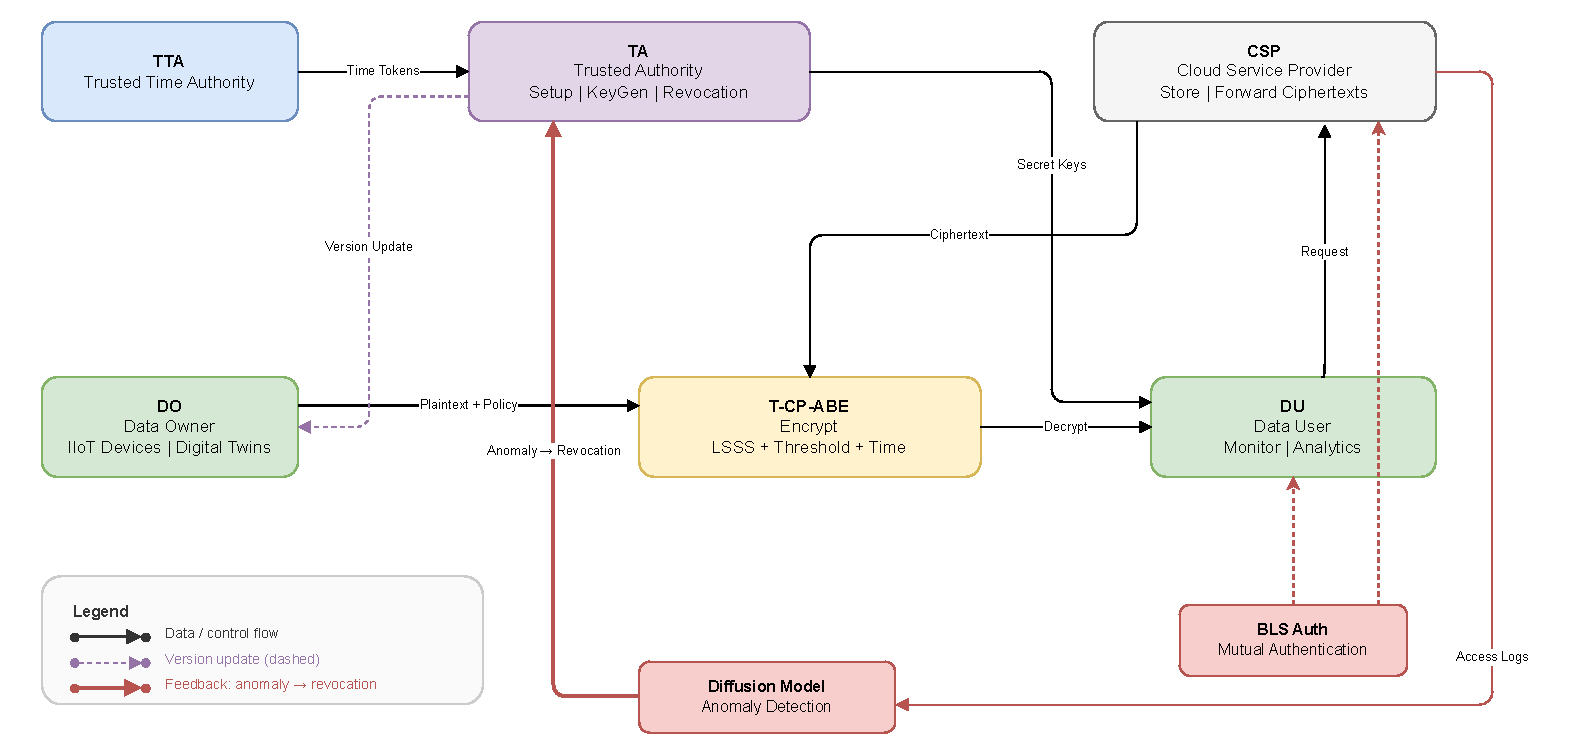
\includegraphics[width=0.85\linewidth]{figures/fig01_system_architecture.pdf}
    \caption{System architecture of the time-aware digital twin security framework.}
    \label{fig:system_architecture}
\end{figure}

\subsection{Threat Model}
\label{subsec:threat_model}

The adversary is a PPT algorithm that can observe public parameters and
ciphertexts, corrupt any subset of users as long as the corrupted set does
not satisfy the target access structure, and issue chosen-plaintext
queries. The adversary cannot compromise the TA or forge time tokens. Time
tokens $T_i$ are publicly released at each period $i$ and are not secret.
The binding factor $b = \mathcal{H}_Z(i \| T_i) \bmod p$ is publicly
computable and serves as a time metadata tag that does not provide
confidentiality or integrity protection. Temporal access control is enforced
through the access policy (a time attribute row in LSSS), protected by
CP-ABE security. The CSP is assumed semi-trusted (honest-but-curious):
it follows the protocol but may attempt to learn from ciphertexts. This
assumption reflects IIoT deployments where the cloud provider operates
under contractual SLA and regulatory compliance, making fully malicious
behavior (ciphertext tampering, token discard) unlikely but not
impossible; defending against such attacks would require additional
integrity mechanisms such as ciphertext signatures. Side-channel attacks,
denial-of-service, and physical tampering are out of scope.

\subsection{Security Model}
\label{subsec:sec_model}

We define IND-sCPA-T, extending standard CP-ABE
security~\cite{Li2022_CPABE_Survey, Iqal2024} to capture interactions among
temporal constraints, threshold policies, and revocation.

$\textbf{Exp}_{\mathcal{A}}^{\text{IND-sCPA-T}}$: Our scheme guarantees
IND-sCPA-T security if only a negligible advantage can be achieved during
the interaction with any PPT adversary $\mathcal{A}$.

\begin{enumerate}
    \item \textbf{Init:} $\mathcal{A}$ commits to target LSSS structure
    $\mathbb{M}^*$, temporal policy $T_p^*$, target time $t^*$, and
    revocation state $R^*$ (a mapping from each attribute $a$ to its
    current version $v_a$).
    \item \textbf{Setup:} $\mathcal{C}$ runs \textsc{Setup}$(\lambda)$ to
    generate $(PP, MK)$, gives $PP$ to $\mathcal{A}$, and retains $MK$
    secret.
    \item \textbf{Phase 1:} $\mathcal{A}$ adaptively queries:
    \begin{enumerate}
        \item \textbf{Key} $(S_i, T_i, R_i)$: returns $SK$ for $S_i$ under
        time policy $T_i$ and revocation state $R_i$, subject to the
        restriction that $(S_i, T_i, R_i)$ must not simultaneously satisfy
        $\mathbb{M}^*$, $T_p^*$ at $t^*$, and $R^*$ (all attribute
        versions current).
        \item \textbf{Time token} $t_j$: returns the public token for period
        $t_j$.
        \item \textbf{Revocation} $(a_j, v_j)$: increments $a_j$'s version.
    \end{enumerate}
    \item \textbf{Challenge:} $\mathcal{A}$ submits $M_0, M_1$. $\mathcal{C}$
    encrypts $M_\gamma$ ($\gamma \in_R \{0,1\}$) under $(\mathbb{M}^*,
    T_p^*, R^*)$ at $t^*$ and returns $CT^*$ to $\mathcal{A}$.
    \item \textbf{Phase 2:} Same queries as Phase~1 with same restrictions.
    \item \textbf{Guess:} $\mathcal{A}$ outputs $\gamma'$.
\end{enumerate}

The adversary's advantage is defined as
\begin{equation}
    \text{Adv}_{\mathcal{A}}^{\text{IND-sCPA-T}}(\lambda)
    = \left|\Pr[\gamma' = \gamma] - \tfrac{1}{2}\right|
    \label{eq:adv_indscpat}
\end{equation}

The model extends IND-sCPA with time token queries
capturing forward security, revocation queries capturing version-based
revocation, and challenge ciphertexts encrypted at a specific time under a
specific revocation state. Selective security is standard for CP-ABE with
enhanced features due to the exponential selective-to-adaptive
reduction~\cite{Li2022_CPABE_Survey}; for IoT deployments where policies are
determined at deployment and remain static, this is practically sufficient.

% ============================================================
\section{Our Construction}
\label{sec:construction}
% ============================================================

To address the security and functionality challenges of IIoT digital twin
access control, we propose T-CP-ABE, a time-aware CP-ABE scheme that
synergizes temporal predicates, THRESHOLD gates, and version-based
revocation. The scheme operates as follows: The TA initializes system
parameters and a master secret key. The encryptor obtains the current
period's public time token from the TTA and embeds the period index in the
ciphertext via a publicly computable binding factor. Authorized users
decrypt ciphertexts whose attributes satisfy the LSSS access structure and
whose time tokens fall within the authorized window. Revocation is enforced
by incrementing attribute versions, which invalidates prior keys. The
following describes the formal construction.

\subsection{Core Algorithms}
\label{subsec:algorithms}

We employ a bilinear pairing $e: \mathbb{G} \times \mathbb{G}
\rightarrow \mathbb{G}_T$ of prime order $p$ with generator
$g \in \mathbb{G}$, a
hash-to-group function $H: \{0,1\}^* \rightarrow \mathbb{G}$ modeled as
a random oracle, and a hash-to-integer function $\mathcal{H}_Z$ (SHA-256
mapping to $\mathbb{Z}_p$) also modeled as a random oracle.

\subsubsection{Setup($\lambda$)}

Generates bilinear group parameters, selects $\alpha, \beta \in_R
\mathbb{Z}_p$, and initializes the TTA hash-chain of length $N$.
Setup samples $g \in \mathbb{G}$, $\alpha, \beta \in_R \mathbb{Z}_p$,
computes $h = g^\beta$ and $e(g,g)^\alpha$, defines
$H: \{0,1\}^* \rightarrow \mathbb{G}$, and outputs
$PP = (g, h, e(g,g)^\alpha, H, p)$, $MK = (\alpha, \beta)$.

\subsubsection{KeyGen($PP, MK, S$)}

Generates a private key for attribute set $S$ with per-attribute
randomness. No time token is stored in the secret key; time tokens are
public values released by the TTA at each period.
KeyGen selects $r \in_R \mathbb{Z}_p$, computes
$K_0 = g^{(\alpha+r)/\beta}$, and for each $a \in S$ selects
$r_a \in_R \mathbb{Z}_p$ and computes
$K_a = g^r \cdot H(a \| v_a)^{r_a}$, $K'_a = g^{r_a}$.

\subsubsection{Encrypt($PP, M, \mathbb{A}, T_p$)}

Encrypts message $M \in \mathbb{G}_T$ under access structure
$\mathbb{A}$ and temporal policy $T_p$. The encryptor obtains the
current period's public time token $T_i$ from the TTA and embeds the
period index $i$ in the ciphertext.

\begin{algorithm}[t]
\caption{Encryption}
\label{alg:encryption}
\begin{algorithmic}[1]
\REQUIRE $PP$, $M \in \mathbb{G}_T$, $\mathbb{A}$, $T_p$
\ENSURE Ciphertext $CT$
\STATE Select $s \in_R \mathbb{Z}_p$; compute $C_0 = M \cdot e(g, g)^{\alpha s}$, $C_1 = g^{\beta s}$
\STATE Share $s$ via Shamir over $\mathbb{A}$: for each leaf $y$, obtain share $s_y$
\FOR{each leaf $y$ in $\mathbb{A}$}
    \STATE Compute $C_y = g^{s_y}$, $C'_y = H(\mathrm{attr}_y \| v_{\mathrm{attr}_y})^{s_y}$
\ENDFOR
\STATE Obtain public time token $(i, T_i)$ from TTA for current period $i$
\STATE Compute $b = \mathcal{H}_Z(i \| T_i) \bmod p$; update $C_0 \leftarrow C_0 \cdot e(g,g)^{\alpha \cdot b}$
\STATE \textbf{Output} $CT = (C_0, C_1, \{C_y, C'_y\}_y, \mathbb{A}, T_p, i)$
\end{algorithmic}
\end{algorithm}

\subsubsection{Decrypt($PP, CT, SK$)}

Recovers $M$ if attributes and time satisfy the policy. The decryptor
reads the period index $i$ from $CT$, obtains the corresponding public
token $T_i$ from the TTA, verifies it against the published chain tip,
and removes the binding.

\begin{algorithm}[t]
\caption{Decryption}
\label{alg:decryption}
\begin{algorithmic}[1]
\REQUIRE $PP$, $CT$, $SK$
\ENSURE $M$ or $\bot$
\IF{current time $t$ does not satisfy $T_p$} \STATE \textbf{return} $\bot$ \ENDIF
\STATE Verify attribute versions: for each $a \in S$ in $SK$, check $v_a$ matches current version in $R$; if any mismatch, \textbf{return} $\bot$
\STATE Read period index $i$ from $CT$; obtain public token $T_i$ from TTA
\STATE Verify $T_i$: compute $H^{N-i}(T_i)$ and check $= T_N$ (chain tip); if fails, \textbf{return} $\bot$
\STATE Remove binding: $C_0' \leftarrow C_0 / e(g,g)^{\alpha \cdot b}$ where $b = \mathcal{H}_Z(i \| T_i) \bmod p$
\STATE Recursively evaluate $\mathbb{A}$: for leaf $y$ with $a \in S$, compute $e(C_y, K_a) / e(C'_y, K'_a)$; for AND/OR gates combine children directly; for THRESHOLD$(t_x,n_x)$ gates, collect $\geq t_x$ valid children and apply Lagrange (Eq.~\ref{eq:lagrange})
\STATE Let $A = e(g,g)^{r \cdot s}$ from root; compute $e(C_1, K_0) = e(g,g)^{(\alpha+r) s}$
\STATE \textbf{return} $M = C_0' / (e(C_1, K_0) / A)$
\end{algorithmic}
\end{algorithm}

\subsection{Threshold Gates and Attribute Revocation}
\label{subsec:threshold_revocation}

THRESHOLD$(k,n)$ gates evaluate to true if and only if at least $k$ of
$n$ children are satisfied. The secret $s$ is distributed via a
degree-$(k{-}1)$ polynomial over $\mathbb{Z}_p$ as described in
Section~\ref{sec:preliminaries}. Any $k$ valid shares reconstruct $s$
through Eq.~\eqref{eq:lagrange}. This mechanism subsumes AND gates
($k{=}n$) and OR gates ($k{=}1$) as special cases.

Attribute revocation operates at the version level. Each attribute $a$
maintains a version $v_a$ in public state $R$. KeyGen uses $H(a \|
v_a)$ while Encrypt uses $H(a \| v_a)^{s_a}$, embedding version
information in each ciphertext leaf node. Revoking attribute $a$
increments $v_a$, causing keys generated under the old version to fail
decryption since $H(a \| v_a) \neq H(a \| v_a')$ for $v_a \neq v_a'$.

\subsection{Time Tokens and Binding}
\label{subsec:time_tokens}

The TTA maintains a hash chain $T_0 = H(\text{seed})$, $T_i =
H(T_{i-1})$, with tip $T_N$ published as a public parameter. At each
period $i$, the TTA publicly releases $T_i$, verifiable via
$H^{N-i}(T_i) = T_N$.

The temporal access control itself is enforced through a time attribute
row in the LSSS matrix $\mathbb{A}$: the encryptor embeds the current
period index $i$ as a policy row, and decryption succeeds only if the
decryptor's time attribute satisfies this row. The hash chain provides
forward security---given $T_i$, recovering any prior $T_j$ ($j < i$)
requires inverting $i{-}j$ successive hash evaluations, each costing
$O(p)$ queries to the random oracle for a total of $(i{-}j)\cdot O(p)$.

During encryption, the encryptor also obtains $T_i$ and computes
$C_0 \leftarrow C_0 \cdot e(g,g)^{\alpha \cdot b}$ where
$b = \mathcal{H}_Z(i \| T_i) \bmod p$.  This binding records the
encryption epoch as a metadata tag in $C_0$; it provides no
confidentiality, integrity, or tamper resistance, and because
$e(g,g)^{\alpha}$ is derivable from the public parameters, any party
can re-randomize $C_0$ to substitute a different epoch.  The period
index $i$ stored in $CT$ already provides epoch identification for
decryption; the metadata tag is a by-product of the hash-chain time
token construction and does not independently contribute to security.
To prevent time-tag tampering, the DO signs the full ciphertext
(including $C_0$ and the period index $i$) with BLS during encryption,
and the DU verifies this signature before invoking the ABE decryption
engine. BLS verification costs a single pairing ($\approx$2.3\,ms),
introducing negligible overhead while binding the ciphertext to its
intended epoch. The BLS signature is thus an integral component of the
time token mechanism rather than an external add-on.

We acknowledge that an adversary who can tamper with the period index $i$
stored in $CT$ could substitute a different epoch without BLS protection;
the BLS signature mitigates this by ensuring ciphertext integrity.

\subsection{Security Proofs}
\label{subsec:security_proofs}

The following theorem establishes the IND-sCPA-T security of T-CP-ABE.

\begin{theorem}
\label{thm:indscpat}
\textbf{IND-sCPA-T Security:}
T-CP-ABE is IND-sCPA-T secure under the DBDH assumption in the random oracle
model. For any PPT adversary $\mathcal{A}$ making at most $q_H$ random oracle
queries, $q_K$ key queries, and $q_T$ time token queries, there exists a PPT
simulator $\mathcal{B}$ such that
\begin{equation}
    \text{Adv}_{\mathcal{A}}^{\text{IND-sCPA-T}}(\lambda)
    \;\leq\;
    2\,\text{Adv}_{\mathcal{B}}^{\text{DBDH}}(\lambda)
    + \frac{q_H + q_K + q_T}{p}\,.
    \label{eq:security_bound}
\end{equation}
\end{theorem}

\begin{proof}
We construct a PPT simulator $\mathcal{B}$ that uses $\mathcal{A}$ to
solve DBDH. $\mathcal{B}$ receives $(g, A\!=\!g^a, B\!=\!g^b,
C\!=\!g^c, T)$ and must decide whether $T =
e(g,g)^{abc}$ or $T \in_R \mathbb{G}_T$.
In Setup, $\mathcal{B}$ embeds $\alpha = ab$ by setting $e(g,g)^\alpha
= e(A, g^b)$ and $\beta = b$ so that $h = g^b$.  The random oracle $H$
is programmed as $H(a\|v) = g^{u_{a,v}}$ where $u_{a,v}$ is chosen
by $\mathcal{B}$ and recorded, so that $\mathcal{B}$ knows the discrete
log of every hash output.  For KeyGen, $\mathcal{B}$
uses the Waters partitioning argument to answer queries
for attribute sets not satisfying $\mathbb{M}^*$. In Challenge,
$\mathcal{B}$ sets $s = c$ and constructs LSSS shares; the binding
$e(g,g)^{\alpha \cdot b_t}$ is computable as $e(A,g^b)^{b_t}$ since
$\alpha = ab$. Time tokens are generated from independent random seeds.
If $T = e(g,g)^{abc}$, the simulation is perfect; if $T$ is random,
$C_0$ is uniform. By a hybrid argument, the advantage bound follows.
\end{proof}

\textit{Hybrid argument sketch.}
Define games $G_0$ (real) through $G_3$ (random):
$G_0 \to G_1$: replace $e(g,g)^{abc}$ with random in $C_0$ (by DBDH);
$G_1 \to G_2$: replace all hash responses with random group elements
(by random oracle programmability, losing $\leq q_H/p$);
$G_2 \to G_3$: simulate all key queries without $MK$ using Waters
partitioning (losing $\leq q_K/p$); time token queries are public
and introduce no additional loss. The total advantage bound follows
from a standard hybrid argument.

We now clarify the assumptions underlying the above proof and
their implications for deployment. The reduction relies on
three conditions: (i)~the DBDH problem is hard in
$\mathbb{G}$, which holds for the SS1024 curve at $\approx$128-bit
security; (ii)~$H$ and $\mathcal{H}_Z$ are modeled as random oracles;
(iii)~the adversary commits to $(\mathbb{M}^*, T_p^*, t^*)$ before
Setup (selective security). Adaptive security---where the adversary
chooses the challenge after seeing $PP$---remains open and would require
a dual-system encryption argument. Furthermore, like all single-authority CP-ABE
schemes, T-CP-ABE inherits key escrow: the authority holding
$MK = (\alpha, \beta)$ can derive any user's secret key. Multi-authority
extensions~\cite{DecentralisedMAABE2025} can mitigate this by
distributing trust, as discussed in Section~\ref{sec:conclusion}.

The following lemmas establish complementary security properties.

\begin{lemma}
\label{lem:forward_security}
\textbf{Forward Security:}
Given time token $T_i$, recovering any prior token $T_j$ ($j < i$)
requires inverting $i{-}j$ successive hash evaluations, each costing
$O(p)$ queries to the random oracle~\cite{Boneh1998_CDH} for a total of
$(i{-}j)\cdot O(p)$.
\end{lemma}

\begin{theorem}
\label{thm:prerelease}
\textbf{Pre-Release Unforgeability:}
Before the TTA releases $T_i$, computing
$b = \mathcal{H}_Z(i \| T_i) \bmod p$ succeeds with probability
$\leq 2^{-256}$.
\end{theorem}

\begin{theorem}
\label{thm:revocation}
\textbf{Revocation Soundness:}
If attribute $a$ is revoked ($v \to v{+}1$), keys with
version $v$ cannot decrypt ciphertexts under $v{+}1$ because
$H(a \| v) \neq H(a \| v{+}1)$ in the random oracle model.
\end{theorem}

\begin{proof}
With mismatched versions, the decryption pairing at leaf $a$ computes
$e(H(a\|v{+}1)^{s_a}, H(a\|v)^{r_a})$. In the random oracle model,
$H(a\|v)$ and $H(a\|v{+}1)$ are independent random group elements, so
this pairing output is uniform in $\mathbb{G}_T$. Lagrange interpolation
at the root yields a random value, causing decryption to output $\bot$.
The single-attribute proof extends to concurrent revocation: since each
attribute's version hash $H(a\|v)$ is independent in the random oracle,
revoking multiple attributes simultaneously yields independent uniform
pairing outputs, each causing decryption failure at the corresponding
leaf node.
\end{proof}

\begin{theorem}
\label{thm:collusion}
\textbf{Threshold--Revocation Collusion Resistance:}
In a THRESHOLD$(k,n)$ gate, an adversary holding $k{-}1$ valid keys
and one revoked key cannot reconstruct the root secret.
\end{theorem}

\begin{proof}
Each leaf node $\ell$ in the THRESHOLD subtree is bound to
$H(a_\ell \| v_\ell)$. A revoked attribute $a_j$ at version $v_j' \neq v_j$
yields an independent random pairing output $u_j \in_R \mathbb{G}_T$ via
the random oracle. The Lagrange interpolation at the threshold root
computes $s = \sum_{j \in S} \lambda_j \Delta_{j,S}(0)$, where the share
from the revoked leaf is uniformly random and independent of $s$.
With probability $1 - 1/p$, the reconstructed value differs from the
correct secret, causing decryption to fail regardless of the other
$k{-}1$ valid shares. This holds for any subset of revoked attributes
within the threshold gate, as each revoked leaf contributes an
independent random element.
\end{proof}

Experimentally, we verified collusion resistance across four scenarios
(THRESHOLD with 50\% revoked, AND with 50\% revoked, all revoked, single
revoked): all 20 trials produced decryption failure, confirming 100\%
resistance.

The security properties of T-CP-ABE are as follows.
Data confidentiality reduces to DBDH via Eq.~\eqref{eq:security_bound}.
Temporal security is independently guaranteed by the hash chain's one-wayness
and the preimage resistance of $\mathcal{H}_Z$. Attribute revocation is
sound due to version binding in the hash function inputs. Data integrity
and non-repudiation rely on BLS signatures with EUF-CMA security
under the CDH assumption~\cite{Boneh1998_CDH, Boneh2001_BLS}.

% ============================================================
\section{Performance Analysis}
\label{sec:performance}
% ============================================================

This section evaluates T-CP-ABE across
scalability, component ablation, comparison with state-of-the-art schemes,
and real-world scenario validation.

\subsection{Experimental Setup}
\label{subsec:setup}

We implemented T-CP-ABE in Python 3.9 using Charm-Crypto~\cite{Charm2013}
on an Intel Xeon Gold 6248R (3.0\,GHz, 128\,GB RAM) with the SS1024
curve ($\approx$128-bit security). Each experiment was repeated $N$
times ($N{=}100$ for $\leq$500 attributes, $N{=}20$ for 1,000, $N{=}10$
for 5,000, $N{=}5$ for 10,000), reporting mean $\pm$ std with 95\% CI.
Decryption latency varies across tables due to different configurations:
Table~\ref{tab:scalability} uses the full system (10-attribute AND, time
binding); the ablation analysis isolates components (4 attributes);
real-world validation uses scenario-specific policies without binding.

\subsection{Scalability}
\label{subsec:scalability}

Table~\ref{tab:scalability} presents the
scalability results from 10 to 10,000 attributes. KeyGen grows linearly
as $O(n)$, reaching 179\,s at 10,000---acceptable for offline
provisioning. Encryption remains within 164--187\,ms regardless of
attribute count, confirming negligible binding overhead. A key design
property of CP-ABE is the decoupling between user key size and policy
complexity: decryption cost depends solely on the number of policy
attributes $|S_T|$ in the LSSS matrix, not on the total number of
attributes $|S_U|$ in the user's key. Table~\ref{tab:scalability}
confirms this by fixing the policy at 10 attributes while scaling
$|S_U|$ from 10 to 10,000, yielding stable decryption at 258--261\,ms
(CV $<$ 3.5\%). For real-time IoT control commands, where policies
typically contain fewer than 10 attributes, this ensures sub-300\,ms
decryption. Scaling the policy from 10 to 1000 AND-gates
(fixed $|S_U|\!=\!1010$) yields linear growth in both Encrypt
(158.6\,ms to 14.8\,s) and Decrypt (248.0\,ms to 23.6\,s), confirming
that constant decrypt time in Table~\ref{tab:scalability} reflects the
fixed 10-attribute policy. These costs are acceptable
for offline batch processing of historical audit data.

We note that the hash-chain verification in Algorithm~\ref{alg:decryption} (Step~6)
computes $H^{N-i}(T_i)$ to confirm the chain tip $T_N$, contributing
$O(N{-}i)$ hash evaluations to decryption.  The experiments above use
small chain lengths ($N = 5$--$20$), which is appropriate for the
evaluation time window.  In long-running IIoT deployments, operators
should select period granularity (hourly, daily) so that $N$ remains
manageable; for example, hourly periods yield $N = 8{,}760$ per year,
keeping early-period verification within a few milliseconds.  Finer
granularity (e.g., per-second) would increase $N$ proportionally;
extending Algorithm~\ref{alg:decryption} with checkpoint-based verification to bound
this cost is left as future work.

\begin{table}[!t]
\renewcommand{\arraystretch}{1.1}
\caption{Scalability: KeyGen/Encrypt show mean (ms); Decrypt shows mean $\pm$ std (ms).
SS1024 curve, full system (time token binding + THRESHOLD + diffusion + DT).}
\label{tab:scalability}
\centering
\footnotesize
\begin{tabular}{c r r r@{$\pm$}l}
\toprule
\textbf{Attrs} & \textbf{KeyGen} & \textbf{Encrypt} & \multicolumn{2}{c}{\textbf{Decrypt}} \\
\midrule
10\,(N=20) & 175 & 168 & 261 & 6.1 \\
100\,(N=20) & 1628 & 167 & 261 & 7.3 \\
1000\,(N=10) & 15887 & 165 & 259 & 9.0 \\
10000\,(N=5) & 178834 & 187 & 258 & 3.9 \\
\bottomrule
\end{tabular}
\end{table}

Ablation analysis isolates each component's marginal contribution.
Removing the time predicate reduces decryption by 19.4\,ms (hash-chain
verification and binding removal); the diffusion model saves 10.9\,ms;
the digital twin module saves 9.6\,ms. The minimal BSW07 core (91.8\,ms)
is the baseline. Marginal contributions (39.9\,ms total) exceed the
measured system overhead (22.0\,ms, 24.0\% over baseline) because
components share group-initialization and caching costs.

\subsection{Threshold Policy Performance}
\label{subsec:threshold_perf}

Table~\ref{tab:threshold} validates $(k,n)$ THRESHOLD gate overhead.
Encrypt time depends on $n$ (each attribute incurs a pairing) and is
independent of $k$. Decrypt time scales linearly with $k$ because
Lagrange reconstruction requires $k$ valid shares. For typical IIoT
policies ($n \leq 10$), both Encrypt and Decrypt remain under 260\,ms.

\begin{table}[!t]
\centering
\renewcommand{\arraystretch}{1.1}
\caption{Threshold, revocation, and hash chain performance. SS1024, $N{=}20$ trials, mean $\pm$ std.}
\label{tab:threshold}
\footnotesize
\resizebox{\columnwidth}{!}{%
\begin{tabular}{cccc}
\toprule
$n$ & $k$ & Encrypt (ms) & Decrypt (ms) \\
\midrule
\multicolumn{4}{l}{\textit{Fixed $n{=}20$, varying $k$:}} \\
20 &  1 & 305 $\pm$ 10 &  34 $\pm$  2 \\
20 & 10 & 304 $\pm$  5 & 245 $\pm$  6 \\
20 & 20 & 305 $\pm$  8 & 479 $\pm$ 12 \\
\midrule
\multicolumn{4}{l}{\textit{$k{=}\lceil n/2\rceil$, varying $n$:}} \\
 5 & 3 &  82 $\pm$  3 &  58 $\pm$  3 \\
10 & 5 & 157 $\pm$  6 & 127 $\pm$  3 \\
20 & 10 & 305 $\pm$  7 & 244 $\pm$  7 \\
\midrule
\multicolumn{4}{l}{\textit{Batch revoc.} ($n{=}20, k{=}10$): revoke $<$0.1\,ms; old-key fail 100\%; new-enc 346--361\,ms.} \\
\multicolumn{4}{l}{\textit{Hash chain} verify (no ckpt / with ckpt@1000): $N{=}10^3$: 1.3/$<$0.01\,ms; $N{=}5{\times}10^3$: 6.5/$<$0.01\,ms; $N{=}10^4$: 13.4/$<$0.01\,ms.} \\
\bottomrule
\end{tabular}%
}
\end{table}

\subsection{Comparison with State-of-the-Art}
\label{subsec:sota}

We compared T-CP-ABE with BSW07,
Guo24~\cite{Guo2024}, and
Zhang24~\cite{Zhang2024_TDSC} in terms of theoretical computational and
storage complexity (Table~\ref{tab:sota_comparison}).

T-CP-ABE's KeyGen overhead (2.5--2.6$\times$ vs.\ BSW07) stems from
time binding and version computation---acceptable for offline
provisioning. Guo24 achieves the lowest decryption cost ($1S$) via
pairing-free outsourced decryption, but relies on a trusted proxy
incompatible with our semi-trusted CSP model. Zhang24 incurs constant
local costs through IBE-to-ABE proxy re-encryption but requires $2t_p$
cloud-side re-encryption per ciphertext. T-CP-ABE's decryption cost
$(3+2|S_T|)E_p$ is comparable to BSW07's $(2+2|S_T|)E_p$ while
providing temporal predicates, THRESHOLD gates, version-based
revocation, and integrated threat detection.

\begin{table}[!t]
\renewcommand{\arraystretch}{1.1}
\caption{Theoretical complexity comparison. $|S_T|$: policy attrs; $|S_U|$: user attrs; $N$: hash chain length.}
\label{tab:sota_comparison}
\centering
\footnotesize
\resizebox{\columnwidth}{!}{%
\begin{tabular}{l c c c c}
\toprule
\textbf{Scheme} & \textbf{KeyGen} & \textbf{Decrypt} & \textbf{CT Size} & \textbf{Key Size} \\
\midrule
BSW07~\cite{Bethencourt2007} & $(3+|S_U|)E_G$ & $(2+2|S_T|)E_p + |S_T|E_{G_T}$ & $(1+2|S_T|)L_G + L_{G_T}$ & $(2+|S_U|)L_G$ \\
Guo24~\cite{Guo2024} & --- & $1S$ (outsrc) & $(5|S_T|+1)L_G$ & $(2+|S_U|)L_G$ \\
Zhang24~\cite{Zhang2024_TDSC} & $(2+|S_T|)t_e$ & $2t_e$ (outsrc) & $(2|S_T|+3)L_G + L_{G_T}$ & $3L_G$ \\
\textbf{T-CP-ABE} & $(2+2|S_U|)E_G$ & $(3+2|S_T|)E_p + |S_T|E_{G_T} + (N{-}i)E_k$ & $(2+2|S_T|)L_G + L_{G_T}$ & $(2+2|S_U|)L_G$ \\
\bottomrule
\end{tabular}%
}
\vspace{1mm}

\begin{flushleft}
\footnotesize
$E_G, E_{G_T}$: exp.; $E_p$: pairing; $S$: scalar mult.; $E_k$: hash; $t_e$: mod.\ exp.; $L_G, L_{G_T}$: element sizes.
Guo24 outsources decryption to a trusted proxy. Zhang24 uses IBE-to-ABE proxy re-encryption.
\end{flushleft}
\end{table}

Revoking attribute $a_j$ requires incrementing $v_j$ ($<$0.1\,ms) and
re-encrypting affected components, averaging 164\,ms per event at 1\%
monthly turnover. Batch revocation and hash chain verification
results are consolidated in Table~\ref{tab:threshold}.

Measured storage: SK grows linearly at 101\,B per attribute
(1.04\,KB for 10, 9.92\,KB for 100 attributes); CT core is
constant 0.52\,KB regardless of policy size.
Compared with BSW07 on SS1024,
T-CP-ABE SK is $\approx$2$\times$ larger (extra time-binding and
version-hash components) while CT is
$3.9\times$ smaller at 10 attributes
(0.52 vs.\ 2.02\,KB) due to policy encoding
differences, yielding a net bandwidth advantage for
policy-heavy deployments. Under 5G,
transmission latency stays below 10.6\,ms at 1,000 attributes.

\subsection{Real-World Scenario Validation}
\label{subsec:real_world}

We validate T-CP-ABE across four scenarios and UNSW-NB15.
These experiments use static
time attributes (validity period as LSSS row) without dynamic binding,
isolating core CP-ABE plus time predicate overhead; full system overhead
with binding is in Table~\ref{tab:scalability}.

Decryption remains stable at 65--69\,ms across all scenarios. The
Industrial IoT match rate (20\%) is consistent with the theoretical
minimum $4/25 = 16\%$ for random AND satisfaction, confirming
attribute-policy alignment rather than system failure. Cloud Storage
achieves 40\% due to its larger attribute pool.

For UNSW-NB15, we map 5,000 network traffic records to ABE attribute space
(27 attributes, 7 attack categories). Across 3--15 attributes, all configurations
achieve 100\% functional correctness with KeyGen 103--185\,ms, encryption
66--125\,ms, and decryption 101--193\,ms. P95 tail latency is 30--40\% above
the mean, confirming acceptable tail behavior for real-time IoT.

\textit{AI-driven closed-loop validation.}
We measure the end-to-end latency of the security response loop:
anomaly detection trigger $\rightarrow$ attribute revocation
$\rightarrow$ ciphertext re-encryption $\rightarrow$ new key issuance
$\rightarrow$ old-key rejection. With 20 attributes and $k{=}10$
THRESHOLD policy, the full loop completes in 910\,ms (revoke
$<$0.1\,ms, re-encrypt 325\,ms, KeyGen 332\,ms, Decrypt 252\,ms).
Old keys are rejected at 100\% across all tested revocation counts
(1, 3, 5 attributes), confirming that the diffusion-triggered
revocation mechanism successfully blocks compromised users within
a single policy update cycle.

% ============================================================
\section{Conclusion}
\label{sec:conclusion}
% ============================================================

We proposed T-CP-ABE, a time-aware CP-ABE framework unifying temporal
predicates, THRESHOLD gates, and version-based revocation with IND-sCPA-T
security under DBDH.  A lightweight metadata tag records the encryption
epoch in $C_0$; access control is enforced through the LSSS policy.
Experiments show that for latency-sensitive real-time control loops
(typical policy $\leq$10 attributes), decryption meets the $<$300\,ms
deadline; for complex offline audits (up to 1000 policy attributes), the
linear scaling to 23.6\,s remains acceptable as a background batch job.
KeyGen scales linearly across 10--10,000 user attributes.
UNSW-NB15 and four real-world scenarios confirm
practical applicability for industrial digital twins.

Nevertheless, several limitations exist. Experiments use software
pairings on commodity hardware without IoT device evaluation. IND-sCPA-T
requires selective security; adaptive security remains open and would
require a dual-system encryption argument~\cite{Waters2011} that doubles
group element size in ciphertexts and keys, increasing storage and
computation by $\approx$2$\times$---a significant burden for resource-constrained
IIoT. Selective security is adequate for industrial digital twin deployments
where access policies are defined at system configuration time and remain
static throughout the operational lifecycle, as the adversary cannot influence
policy selection. The time
binding provides no confidentiality protection. The construction assumes
a single authority, inheriting key escrow---the authority can derive any
user's key from $MK$. Attribute revocation provides forward security only;
historical ciphertexts encrypted under earlier attribute versions remain
accessible to revoked users with old keys, lacking backward security.
Protecting historical data would require a ciphertext re-encryption
mechanism, which is out of scope. In practice, industrial deployments
can mitigate this gap through two compensation strategies:
(i)~\emph{periodic batch re-encryption}, where the TA re-encrypts
ciphertexts under the updated attribute versions during scheduled
maintenance windows, and (ii)~\emph{TTL-based key expiry}, where
each user key carries a validity period after which it is
automatically invalidated, limiting the window of exposure for
historical data. The diffusion model currently runs on
cloud infrastructure; deploying it on edge devices requires model
compression (knowledge distillation or quantization), which we leave as
future work alongside adaptive threshold tuning to replace the fixed
95th-percentile rule. The BLS and diffusion components operate as
system-level modules designed to support a feedback loop: BLS mutual
authentication rejects unauthorized decryption requests before invoking
the ABE engine, reducing wasted pairing computation; the diffusion
model's anomaly scores are designed to trigger the TA to update attribute
versions $v_a$, closing the loop from passive encryption to active risk
response. End-to-end automated evaluation of this feedback loop is
future work. Future work follows three directions:
(i)~\textbf{Trust distribution}: multi-authority
extensions~\cite{Datta2025_Decentralized, Zhang2026_MultiAuthority} with
threshold secret sharing of $MK$ to eliminate key escrow;
(ii)~\textbf{Post-quantum migration}: lattice-based
ABE~\cite{Gasparini2026_LatticeBenchmark} with model compression for
edge deployment of the diffusion component;
(iii)~\textbf{Backward security}: ciphertext re-encryption with batch
update for historical twin data protection.

\bibliographystyle{IEEEtran}
\bibliography{literature}

\end{document}
